%%%%%%%%%%%%%%%%%%%%%%%%%%%%%%%%%%%%%%%%%%%%%%%%%%%%%%%%%%%%%%%%%%%%%%%%%%%%%%%
% Chapter 4: Generando un corrector de exámenes: Sinatra renderer
%%%%%%%%%%%%%%%%%%%%%%%%%%%%%%%%%%%%%%%%%%%%%%%%%%%%%%%%%%%%%%%%%%%%%%%%%%%%%%%

%++++++++++++++++++++++++++++++++++++++++++++++++++++++++++++++++++++++++++++++

Este otro \ceit{renderer} genera una \ceit{aplicaci\'on} \ceit{Sinatra} con todo lo necesario para ser desplegada en \ceis{Heroku} o ejecutar localmente. 
Se hace uso de \ceis{Google Drive} para almacenar una copia del \ceit{cuestionario} y para alojar las preguntas y respuestas de los alumnos.

Para usar este renderer es necesario a\~{n}adir especificar algunos par\'ametros m\'as en el fichero \ceit{Ruby} que contiene el cuestionario.
Estos par\'ametros se enumeran a continuaci\'on:

\begin{enumerate}
  \item La direcci\'on de correo en \ceis{Gmail} del profesor. Es posible especificar m\'as de una direcci\'on usando una notaci\'on
  de \ceit{Array}.
  \begin{figure}[!th]
  \begin{center}
  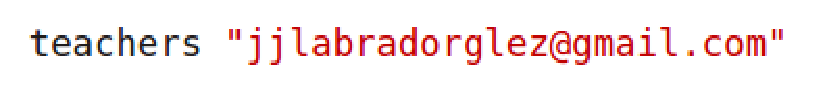
\includegraphics[width=0.5\textwidth]{images/teachers.eps}
  \caption{M\'etodo para especificar los profesores permitidos en la aplicaci\'on}
  \label{fig:teachers}
  \end{center}
  \end{figure}
  
  \item El \ceit{path} de un fichero \ceis{\ref{apend1:csv}} con los datos de los alumnos.
  \begin{figure}[!th]
  \begin{center}
  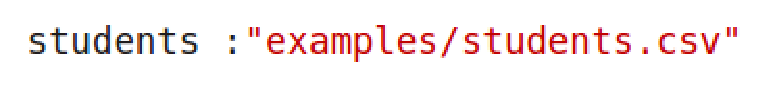
\includegraphics[width=0.5\textwidth]{images/students.eps}
  \caption{M\'etodo para especificar los alumnos permitidos en la aplicaci\'on}
  \label{fig:students}
  \end{center}
  \end{figure}
  \newpage
  
  \item El path de un fichero de configuraci\'on denominado \cei{config.yml} que contiene informaci\'on del cuestionario.
  \begin{figure}[!th]
  \begin{center}
  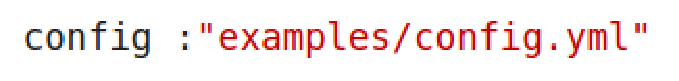
\includegraphics[width=0.4\textwidth]{images/config.eps}
  \caption{M\'etodo para especificar la configuraci\'on de la aplicaci\'on}
  \label{fig:config}
  \end{center}
  \end{figure}
  
\end{enumerate}

Para saber c\'omo rellenar estos par\'ametros, v\'ease Ap\'endice \ref{subsec:Apendice2.12}.
\bigskip

La sintaxis para ejecutar este renderer es la siguiente:
\begin{verbatim}
[~/tmp]$ ruql example.rb Sinatra -t templates/htmlform.html.erb
\end{verbatim}

Tras su ejecuci\'on, se crear\'a una carpeta llamada \cei{app} en el directorio donde nos encontremos. Este \ceit{directorio} contendr\'a lo siguiente:
\begin{figure}[!th]
\begin{center}
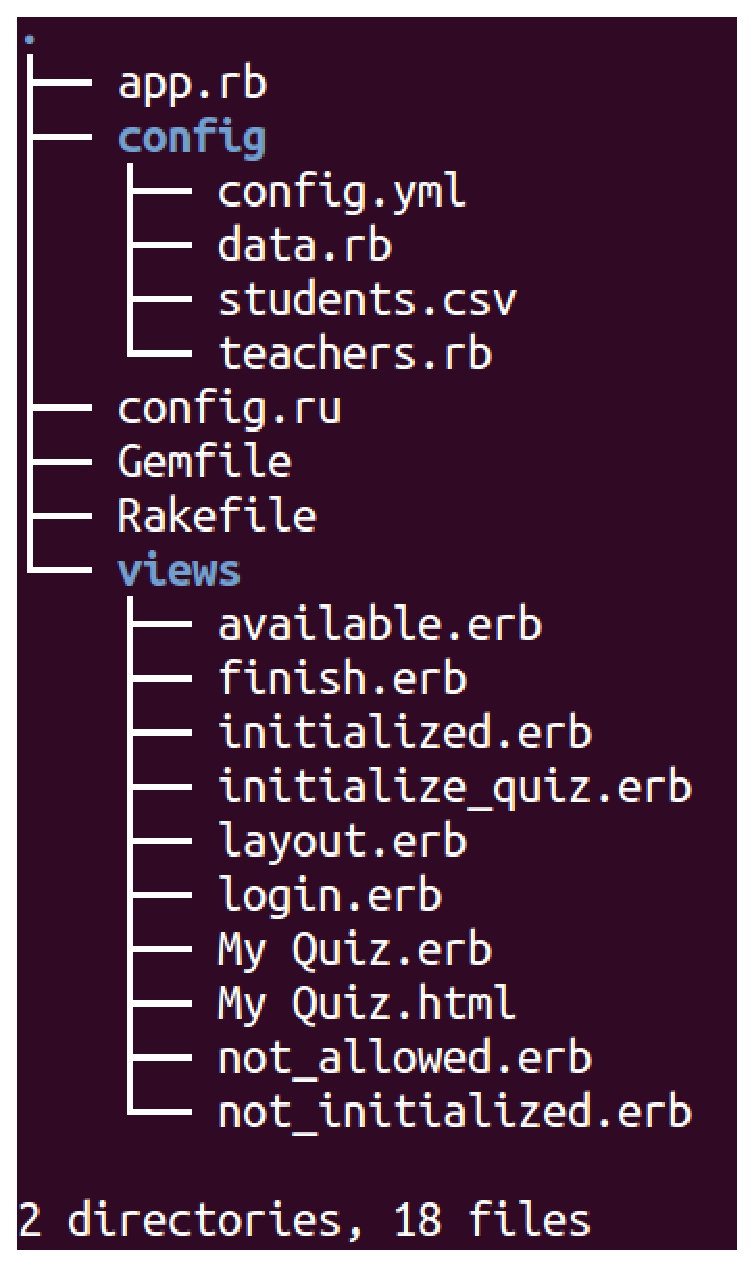
\includegraphics[width=0.4\textwidth]{images/app.eps}
\caption{Listado de ficheros y directorios generado dentro del directorio \textit{app}}
\label{fig:app}
\end{center}
\end{figure}
  
Para obtener informaci\'on de los directorios y ficheros generados, v\'ease Ap\'endice \ref{subsec:Apendice2.15}.
\bigskip
\bigskip
\bigskip

La \ceit{aplicaci\'on} resultante funciona del siguiente modo:
\begin{enumerate}
  \item Una vez ejecutada, el \ceit{profesor} deber\'a autenticarse con su cuenta de \ceit{Gmail} y activar el cuestionario. Hecho esto, se crear\'a en su \ceis{Google Drive} 
  una carpeta que contendr\'a una copia de \ceit{examen} y una hoja de c\'alculo con las preguntas y respuestas correctas del cuestonario. Tambi\'en guardar\'a la informaci\'on
  de los usuarios. 
  
  \item Una vez activido, los alumnos podr\'an acceder a realizar el mismo. Cuando lo finalicen, se generar\'a una copia de su examen en la carpeta de Google Drive del
  profesor y se escribir\'a autom\'aticamente su hoja de c\'alculo para a\~{n}adir la nota que ha sacado el alumno individualmente en cada pregunta y de manera global.
  De este modo, quedar\'a constancia de la realizaci\'on del mismo.
 
  \item Los alumnos podr\'an reintentar el cuestionario todas las veces que deseen mientras se encuentre activo. \'Este dejar\'a de estar activo cuando finalice la fecha 
  l\'{\i}mite establecida por el profesor en el fichero de configuraci\'on. Al reintentar el cuestionario, se actualizar\'a Google Drive con las nuevas calificaciones
  del alumno.
\end{enumerate}

{\bfseries NOTA}: ser\'a responsabilidad del profesor facilitar la nota a los alumnos en el momento que estime oportuno.
\bigskip

Para resolver el gran problema de la \ceit{autentificaci\'on} de usuarios, se hace uso de OAuth. De este modo, delegamos todo el servicio a Google y evitamos, por tanto,
posibles brechas de seguridad que den lugar a suplantaciones de identidad o exposici\'on de datos sensibles de los usuarios a terceras personas. Para poder usarlo
es necesario dar de alta en \ceis{Google Developers Console} una aplicaci\'on. Este proceso se explicar\'a en el apartado del Ap\'endice \ref{subsec:Apendice2.13}.
\bigskip

Un ejemplo completo del funcionamiento de la aplicaci\'on se encuentra en el apartado del Ap\'endice \ref{subsec:Apendice2.16}.
\newpage

%---------------------------------------------------------------------------------
\section{Problemas encontrados y soluciones}
\label{5:sec:1}

\subsection{Timeout corto entre peticiones del navegador al servidor}
\label{subsec:4.1.1}
\bigskip

Al inicializar el cuestionario, el servidor tarda en responder ya que es necesario escribir en \ceit{Google Drive} una cantidad de datos considerable. Cuanto termina la escritura, 
nos debe mostrar una vista en la que se puede comprobar que el cuestionario ha sido inicializado correctamente. Esta vista s\'olo se muestra una vez y \'unicamente al profesor
que inicializ\'o el cuestionario. El resto de ocasiones, se nos redirige al cuestionario en s\'{\i}. 
Sin embargo, mientras se est\'a escribiendo en Google Drive el navegador interpreta que el \ceit{servidor} tarda en responder, por lo que le manda una nueva petici\'on  y \'este la 
despacha en cuanto finaliza la escritura en Google Drive. El problema reside en que atiende a esta nueva petici\'on y, al ver que el cuestionario ya ha sido inicializado,
nos redirige al cuestionario, salt\'andose la vista que deber\'{\i}a aparecer la primera vez.
\bigskip

{\normalsize {\bfseries Soluci\'on}}
\bigskip

Usar como servidor \ceis{\ref{apend1:webrick}} en lugar del que ejecuta Sinatra por defecto (\ceis{\ref{apend1:thin}}). WeBrick no permite m\'ultiples peticiones por lo que se nos muestra la 
vista adecuada al inicializar el cuestionario.

\subsection{Lugar de almacenamiento de las respuestas de los alumnos}
\label{subsec:4.1.2}
\bigskip

Estaba claro que la informaci\'on de los cuestionarios hab\'{\i}a que guardarla en alg\'un lado. La idea principal era almacenar todas las preguntas y respuestas de los alumnos
en una \ceit{base de datos}, pero preocupaba el hecho de que \'esta se alojara en un servidor desconocido y que, por alg\'un motivo, se perdiera dicha informaci\'on sensible.
\bigskip

{\normalsize {\bfseries Soluci\'on}}
\bigskip

Viendo la evoluci\'on que ha tenido la herramienta Google Drive y el aumento considerable de su uso por parte de docentes, decid\'{\i} sustituir las tradicionales y siempre mon\'otonas 
consultas a bases de datos por esta herramienta de \ceit{almacenamiento} que permite visualizar y administrar f\'acilmente toda la informaci\'on. Adem\'as de ser segura, la informaci\'on 
reside en la cuenta del profesor y \'este la puede exportar donde desee c\'omodamente.

\subsection{Problema de seguridad al evaluar c\'odigo Ruby en el servidor}
\label{subsec:4.1.3}
\bigskip

En esta primera versi\'on del \ceit{renderer}, la aplicaci\'on generada eval\'ua el \ceit{c\'odigo} introducido por el alumno sin ning\'un mecanismo de \ceit{protecci\'on}, por lo que introduciendo
alg\'un \ceit{script} comprometedor en el campo de alguna respuesta se podr\'{\i}a comprometer la informaci\'on de la \ceit{aplicaci\'on}.

Este es un aspecto importante a tratar en pr\'oximas mejoras del renderer.
